\chapter{Prospects for Neutral MSSM Higgs Search Improvement}

The neutral MSSM Higgs search, described in the previous chapter, 
suffers strongly of poor jet reconstruction efficiency and  b-tagging performance due to the particular phase space
required, this bound the potential of this search, improoving b-tagging
would result in a major improvement of the search sensitivity. 
This chapter investigates an alternative to the commonly used calorimeter jets in ATLAS, 
which is trackjets b-tagging. 
The prospects for successfully use trackjets b-tagging in the future neutral MSSM Higgs searches are reported,
b-tagging on trackjets was never attempted before.
Section\ref{bla} describes this and that...


\clearpage

\section{Introduction to Trackjets}
% reasonable intro + ++ 
This problematic has two sources:
- The ATLAS calorimeter is not a sampling calorimeter, this means that responses differently 
for Hadrons and for leptons, has different responses to electromagnetic and hadronic shower.
The Calorimeter cells are calibrated in energy using response to electromagnetic showers, to 
know the energy of the original parton that initiated the jet there are different procedure 
to calibrate the Jets offline which are called in short Jet Energy Scale (JES) corrections \cite{}, 
which make use of MC simulation.
Due to the high amount of pileup and ambient energy density in the events, jets are calibrated % also other problems: underlying event ecc..
from 20 GeV in $\pt$, this means that currently is not possible with calorimeter jets to access the
low transverse momentum phase space.

\begin{figure}[tp]
     \begin{center}

            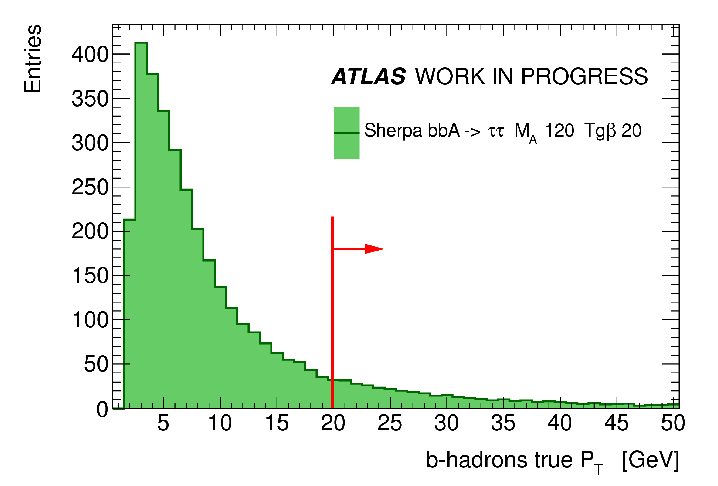
\includegraphics[width=0.49\textwidth]{figure/trackjet/bbA_pt.png}
            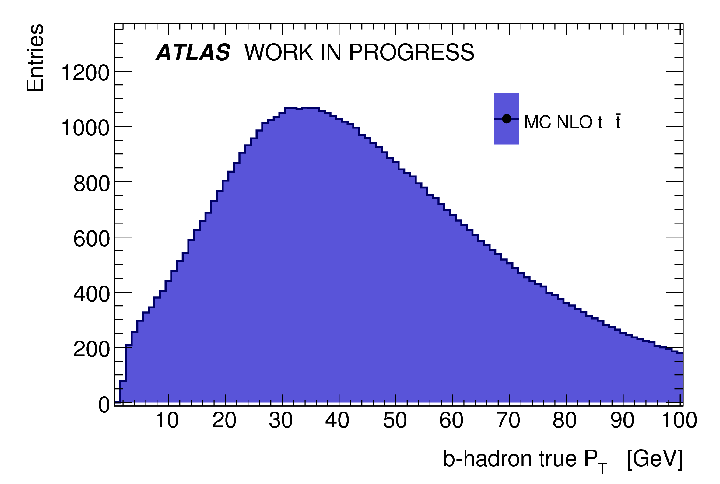
\includegraphics[width=0.49\textwidth]{figure/trackjet/top_pt.png}

    \end{center}
    \caption{Cormparison of simulated b-hadron distribution for signal b-associated production events (left) and $\ttbar$ events (right).
	The red line in the figure shows the acceptance region due to calibrated jet $\pt$ requirements.}
   \label{fig:bjetDistro}
\end{figure}

The neutral MSSM Higgs search, as described in chapter~\ref{chap:anal}, splits the dataset in two category
by means of the presence or the absence of a b-tagged jet, the b-tagged category is optimized for the b-associated production 
mechanism, in which the Higgs is produced in association with two b-jets. Figure~\ref{fig:bjetDistro} shows a comparison 
between $\pt$ spectrum of simulated b-hadron in b-associated Higgs  and $\ttbar$ events, the signal prefers b-hadron with 
relatively low transverse momentum,  jet calibration invoqe jet $\pt > 20$ GeV removing a large fraction of possible
signal candidate, many of the b-associated production signal events falls in fact in the b-veto category, making 
the separation not so effective.
The low $\pt$ spectrum is actually quite challenging, jet reconstruction efficiency and calibration set then a lower limit
to the signal sensitivity in the b-tag category.
Another challenge to this search are the poor b-tagging performance at low transverse momentum, for the a fixed tagging point of the 
MV1 tagger the b-tagging efficiency drops, in fact,  rapidly  with jet $\pt$ reacing a minimum of 50\% at 20 GeV \cite{BtaggingScaleFactors,BtaggingScaleFactorsNew}
(using as tagging point the 70\% point).

A solution to the jet reconstruction efficiency is to use, instead of calorimetric jets (calo-jet), track-jet , which are as well
anti-kt object (see chapter\ref{chap:detector}) but constructed using inner detector tracks as building blocks, not calorimeter cells.
Jets in the ATLAS reconstruction software are reconstructed by clustering foru vector objects (calorimeter energy cluster, tracks, 
truth particle, etc.) in the $\eta - \phi$ plane. In the case of clustering tracks, however, it is possible to take advantege of
the longitudinal (\emph{z}) impact parameter information provided by the inner detector and build track-jets in three dimensions 
$\eta - \phi - z$. Track-jets will then contains only tracks originating from the same interaction point (reconstructed vertex).
Even thoug for calorimeter jet is possible to use the JVF, track-jets result to be more resistant to decrease in performance in the
presence of pile-up, thus particolarly important in b-tagging, which depends on the determination of the jet-axis. 
B-tagging has been never tested before on track-jets, in the following, the first study of b-tagging over track-jets performances is reported. 



%as shown if figure~\ref{





%\subsection{Motivation}
%\subsection{Definition of Trackjet}
\section{Trackjet Performance}
\subsection{B-tagging Performance}
\subsection{Comparison Calo-jet Track-jet}
\subsection{Impact of Trackjet to the Analysis} % A new Hope
\subsection{B-Discriminant} % variable to enhance low pT b-tagging

\section{Systematic Uncertainties on Trackjets}
\subsection{General discussion}
\subsection{Track Subtraction Method} %general description of the method
\subsection{Track Subtraction Validation} %confermo che l'effetto di Ex material e' solo efficiency
\subsection{Track Subtraction Results}

